  \documentclass[12pt]{article}
 
\usepackage[margin=1in]{geometry}
\usepackage{amsmath,amsthm,amssymb}
\usepackage[spanish]{babel}
\decimalpoint
\usepackage{hyperref}
\usepackage[utf8]{inputenc}
\usepackage{enumitem, kantlipsum}
\usepackage{graphicx}
\setlength{\parindent}{0cm} 

\begin{document}
 
\begin{center}
\Large \textbf{C.Física Moderna: Ejercicios Desafío}\\
\normalsize \textbf{Mecánica relativista}
\end{center}
 
  

\section{Dispersión de Compton}

En el efecto Compton se tiene un fotón con longitud de onda $\lambda$ que colisiona con un electrón libre y en reposo. El fotón luego de la colisión tiene una longitud de onda  $\tilde{\lambda}$ y esta dispersado con ángulo $\theta$. El electrón también es dispersado un ángulo $\varphi$. Use $m$ para la masa del electrón.


\begin{figure}[h]
	\centering
	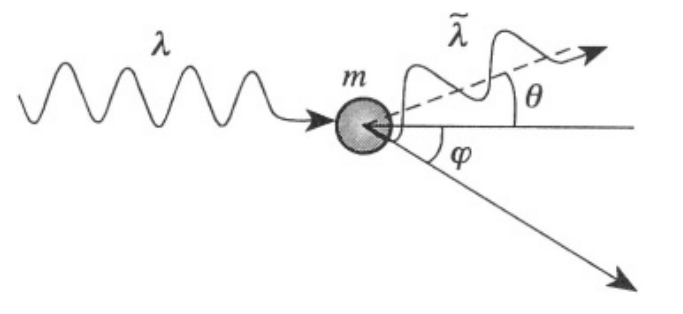
\includegraphics[width=13cm]{compton}
\end{figure}

\begin{enumerate}
	\item Escriba las ecuaciones relativistas de conservación de momento y energía. 
	\item Encuentre una expresión para el cambio de longitud de onda $\Delta \lambda = \tilde{\lambda} - \lambda$ para el caso $\theta = \pi/2$.
\end{enumerate}



\noindent\rule{16.5cm}{0.4pt}





\section{Creación de partículas}

Un fotón con energía $\varepsilon_{\gamma}$ colisiona con un protón estacionario. Para un valor suficientemente grande de  $\varepsilon_{\gamma}$, se produce un mesón $\pi$ en la siguiente reacción:

$$ \gamma + p \rightarrow p + \pi^0 $$   

¿Cuál es la energía $\varepsilon_{\text{min}}$ para que ocurra la reacción?\\

\textbf{Pista:} Use el invariante de momento/energía.\\
\noindent\rule{16.5cm}{0.4pt}

\section{Decaimiento de una partícula}


Considere una partícula A que se encuentra en reposo, y que tiene masa $m_A$. Dicha
partícula decae en otras dos partículas B y C, cuyas masas en reposo son, respectivamente,
$m_B$ y $m_C$. 



\begin{enumerate}
	\item Encuentre las energías de las partículas B y C luego del decaimiento.
	\item Calcule $|\vec{p}_B|$ y $|\vec{p}_C|$.
	\item ¿Qué sucede si $m_A < m_B + m_C$?
\end{enumerate}


\noindent\rule{16.5cm}{0.4pt}



\section{Efecto Doppler Transverso}

Una diferencia cualitativa entre la mecánica clásica y la relatividad es la existencia del efecto Doppler transverso en la relatividad(cuando la luz se propaga en una dirección transversa a la dirección de la fuente visto desde el marco del observador).  Calcule la frecuencia $\omega'$ de un fotón vista por un observador en términos de la frecuencia $\omega$ que emite en reposo y la rapidez relativa entre la fuente y el observador. Para ello piense que el vector de onda y la frecuencia tienen transformaciones análogas a las del espacio-tiempo. En particular la frecuencia tiene la siguiente transformación para una fuente moviéndose en la dirección $x$:

\begin{align*}
\omega= \gamma\left(\omega' - v k_x'\right)
\end{align*} 

Donde $k_x'$ es el numero de onda en la dirección de propagación de la fuente.

Para ver una animación del el efecto Doppler: \url{https://youtu.be/hnphFr2Iai4?t=33s} 



\noindent\rule{16.5cm}{0.4pt}




\end{document}